\chapter{Design}

\section{Analysis of Relevant Technologies}
Determing what programming language(s) and framework(s) to use in a project implementation is an important decision process. A chosen technology must be runnable within the constraints defined in Appendix \ref{Operating Environment}, and ideally should be a technology that the development team, in this case a solo developer, is familiar with as to minimise excessive amounts of time learning.

On the other hand, there is an important balance that must be struck between choosing a tool that is familiar, and that which is most effective, as argued by Vinegar who states that 'writing quality, sustainable software comes second to fiddling with what's sexy'. \cite{Vinegar1}

Ultimately, the languages were refined down to PHP, Node.js, and Python, as they are all comfortably understood by the developer, appropriate for the task of constructing a full-stack web application, and should run on the designated GNU/Linux system environment without issue.

\subsection{PHP}
PHP, otherwise known by the recursive acronym PHP Hypertext Preprocessor, is one of the most famous and important programming languages on the Internet, originally written in 1994 by Rasmus Lerdorf. It can be used in a procedural or object-oriented style, and is allegedly used on more than 20 million websites today. \cite{Wolfe1}

While PHP can be used on its own to great success, there are numerous frameworks available that build on top of PHP to make it better suited for producing full-stack web monoliths that will likely require the use of the popular Model View Controller (MVC) design pattern. This design pattern is described in greater detail in Design Patterns.

The most popular framework of this nature is Laravel, originally conceived by Arkansas developer Taylor Otwell, who in around 2011 was unhappy with the most popular framework at the time, CodeIgniter. \cite{OBrien1} Today, it features a range of features such as built-in authorisation and authentication, MVC clearly built-in as the core design pattern in mind, security mitigations, and most notably, abstracts a lot of the complex database work that would be required in this project behind an Object-Relational Mapper (ORM) called Eloquent, heavily based on ActiveRecord that is found in Ruby on Rails. This functionality would drastically simply development efforts and reduce the quantity of boilerplate code that would need to be written, when the framework can simply be leveraged instead. \cite{Shah1} \cite{Laravel1}

\subsection{Node.js (JavaScript)}
JavaScript, sometimes referred to as ECMAScript due to standards specifications it conforms to,\cite{Mozilla1} was famously written in 10 days by then Netscape employee Brendan Eich for use on the Internet as a client-side, browser interpreted language. \cite{Buytaert1} 

Node.js is an implementation of JavaScript on the server-side and outside of the DOM (Document Object Model) found in webpages that was created in 2009, where over the last decade it has been adopted rapidly by organisations big and small as it unifies the choice of language to JavaScript across the entire web stack. \cite{Copes1}

Like PHP, while it can be used on its own (sometimes referred to as 'vanilla'), there exists a range of frameworks that simplify and better purpose Node.js for use in building complex full-stack web applications and RESTful (Representational State Transfer) APIs. (Application Programming Interface) The most popular example of which, is Express, a minimalist and unopinionated (flexible and easily restructured) released in 2010. \cite{Mozilla2}

While Express eases the workload in developing working routing and other components that make up the MVC design pattern, it is as previously mentioned, minimalist. This means that a lot of the complex work such as working with databases, providing security layers, and programming authentication would need to still be carried out, or delegated to additional libraries, further complicating development.

\subsection{Python}
Python is a scripting language that was created in 1990 by Dutch programmer Guido van Rossum. \cite{Python1} Today, it is one of the most popular programming languages in the world, supporting multiple paradigms and is used not only as an introductory language intended for beginners, but also in fields such as machine learning, embedded systems, and of course, web development. \cite{Heath1}

The two most popular Python web frameworks are Flask and Django - with Flask taking an unopinionated, minimalistic, plugin approach like Express does, whereas Django more closely resembles Laravel and Ruby on Rails for its rich features, such as built-in authentication, and the use of an ORM. 

\subsection{Conclusion}
After a substantial amount of consideration, it was decided upon to use Laravel and PHP for use of the project. Whilst JavaScript and Node.js continue to increase in popularity thanks in part to a unification of languages across the entire web stack, allowing for the reuse of libraries and skill sets for development, testing, etc. it would take significantly more time to develop much of the underlying functionality and architecture that would be necessary for powering an MVC web application, due to Express' minimalism and specific design for lightweight APIs and microservices, as opposed to monolithic, full-stack apps.  \cite{DjangovsNode}

Django and Python would be a perfect fit for the application - providing a near identical set of functionality and boilerplating necessary to develop such an application quickly. Ultimately, personal preference and experience with the PHP ecosystem and best practices, including years of prior usage in substantial academic work and personal projects made PHP a more comfortable choice, and as there are no known downsides or impracticalities from opting for said language, it was an easy decision to make, as opposed to unnecessarily familiarising oneself with new technologies when there are looming deadlines for completion of work, as well as needing to demo work and progress to the client on a weekly basis. As written in the Agile Manifesto, working code is the most ideal indicator of progress. \cite{Sierra1} \cite{beck2001agile}

\subsection{Front-End Considerations}
With PHP and Laravel determined as the back-end language and framework of choice, attention must be paid to any necessary design considerations, libraries, or technologies that will be needed on the front-end. Laravel includes Laravel Mix, an implementation of popular JavaScript workflow tool Webpack, which is used to minify any JavaScript or stylesheet code written, as well as to compile superset languages such as Sass into their basic languages (in this case, CSS) so that it can be interpreted by a web browser. By default, the stylesheet markup language Sass, and the JavaScript framework Vue.js are included with Laravel, but they can be readily interchanged with other technologies such as React or Less. \cite{Laravel2}

One of the main requirements put forth by the customer in regards to front-end design is the need for responsive design, that is, for the application to work and present itself seamlessly regardless of viewport size or device specification: i.e. on a computer, tablet, or smartphone. By including Bootstrap 4, a popular CSS and JavaScript framework developed by Twitter which is additionally included in Laravel by default, the application can be made with responsiveness in mind. While it is not necessary and responsiveness can be implemented in plain CSS or Sass, such as by leveraging the new CSS Grid standard, this is arguably not as quick to scaffold and present to a customer, at the cost of the overhead of requiring to download additional styling and code to be executed within the browser. \cite{Laravel3}

\section{Design Patterns}

\begin{figure}[h!]
    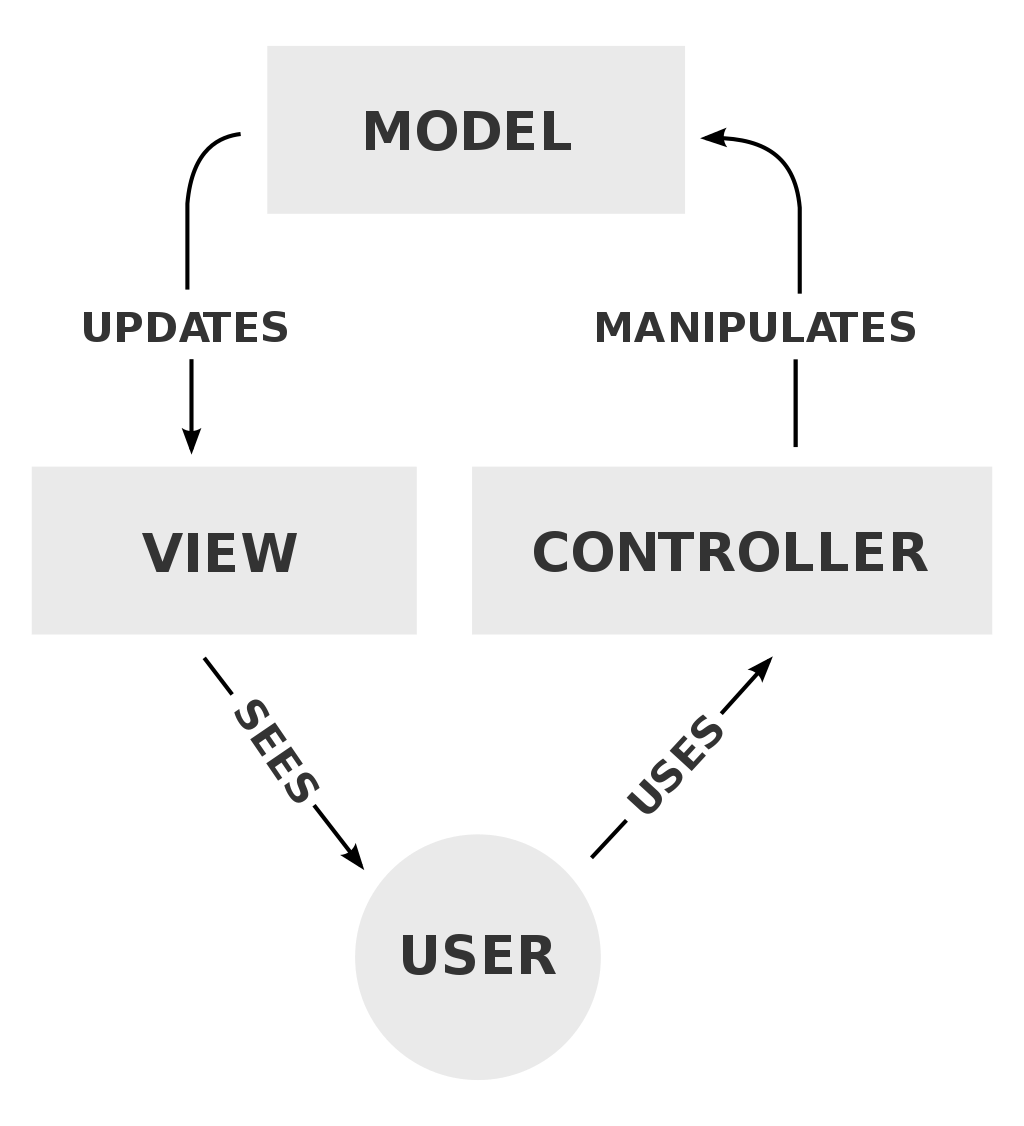
\includegraphics[width=\textwidth]{Figures/mvc}
    \caption{Model View Controller (MVC) Design Pattern}
    \label{fig:mvc1} \cite{mvcimage}
\end{figure}

Laravel, like many application frameworks utilises the Model View Controller architectural pattern in order to help separate concerns and to help compartmentalise code into easily reusable sections. \cite{Ighodaro1} These concerns can be broken down like thus:

\begin{itemize}
    \item The model relates directly due to the data domain, reflecting data held in the database, and almost always is responsible for all actions that involve database access.
    \item The view is what the user sees and interacts with, which can pass instructions back to controllers.
    \item Controllers facilitate communication between the Model and the View, and encapsulate other business logic also. \cite{7892651}
\end{itemize}

It is important to note however, that although Laravel utilises MVC, like many other frameworks, it is does not necessarily consider itself to be such and continues to be a disputed topic in the web development community. \cite{Otwell1} Nevertheless, the application will be developed with this pattern in mind.

\section{Data Persistence}

PHP supports a wealth of relational databases out-of-the-box, and this functionality is extensible with the use of drivers. For development, the use of a SQLite or local MySQL database is more than sufficient, and both Laravel and PHP itself will work wtih different databases without the need for different code or parameters. The PDO (PHP Data Object) is the means in which PHP applications can interface with databases, which fully abstracts away any underlying database mechanisms and allows developers to write fully database agnostic code, without the need of knowing what dialect of SQL, or even writing database queries at all. Resultingly, the customer is free to use whatever database technology they wish, provided that they have the necessary drivers installed on their PHP installation or within their container, such as MySQL, PostgresSQL, or SQLite. \cite{PHP1}

\section{Security Considerations}
An application working with user information, regardless of sensitivity must address certain security considerations in order to conform with the Data Protection Act of 2018, which includes the ability for users to view, edit, and delete aspects of their personal information. This was updated that year to include the British implementation of the European General Data Protection Regulation (GDPR) which has come into effect as the United Kingdom withdraws from the European Union. Charities are not exempt from this legislation. \cite{HMGovt1} \cite{HMGovt2}

It is a well-established concept in software engineering that data from a client (i.e. data from a user) cannot be trusted and must be properly sanitised and validated in order to protect underlying data systems from invalid input, especially malicious input designed to bring harm to data or the systems containing it, such as by means of a SQL Injection attempt - manipulating data inputs to run arbitrary SQL code. \cite{CorePHPProgramming} \cite{Microsoft2}

A wealth of functionality exists within Laravel and will be leveraged in order to mitigate security risks as aforementioned, including full validation and authorisation checks, automatic escaping of data retrieved from database, and CSRF (Cross Site Request Forgery) protection. Passwords are also automatically encrypted when stored in the database and remain so when accessing the user model, providing additional protection. \cite{Laravel4} \cite{Laravel5}

\section{Development Environment}
The application in a macOS (UNIX) environment, on a desktop computer with the following specifications:

\begin{itemize}
    \item Mac Pro (Early 2008)
    \item macOS 10.3.6 High Sierra Operating System
    \item 2 x 2.8GHz Quad Intel Xeon E5462 Processors
    \item 32GB 667MHz Random-Access Memory (RAM)
    \item NVIDIA GeForce GTX1050 Ti Graphics Card
    \item Solid-State Drive
\end{itemize}

Software development is carried out using JetBrains PhpStorm IDE (Integrated Development Environment) thanks to its powerful Laravel and PHP code analysis and refactoring tools that are provided out-of-the-box, making it the most specialised program compared to standard code editors. \cite{Jetbrains1}

\section{Use Case Design}

\begin{figure}[h!]
    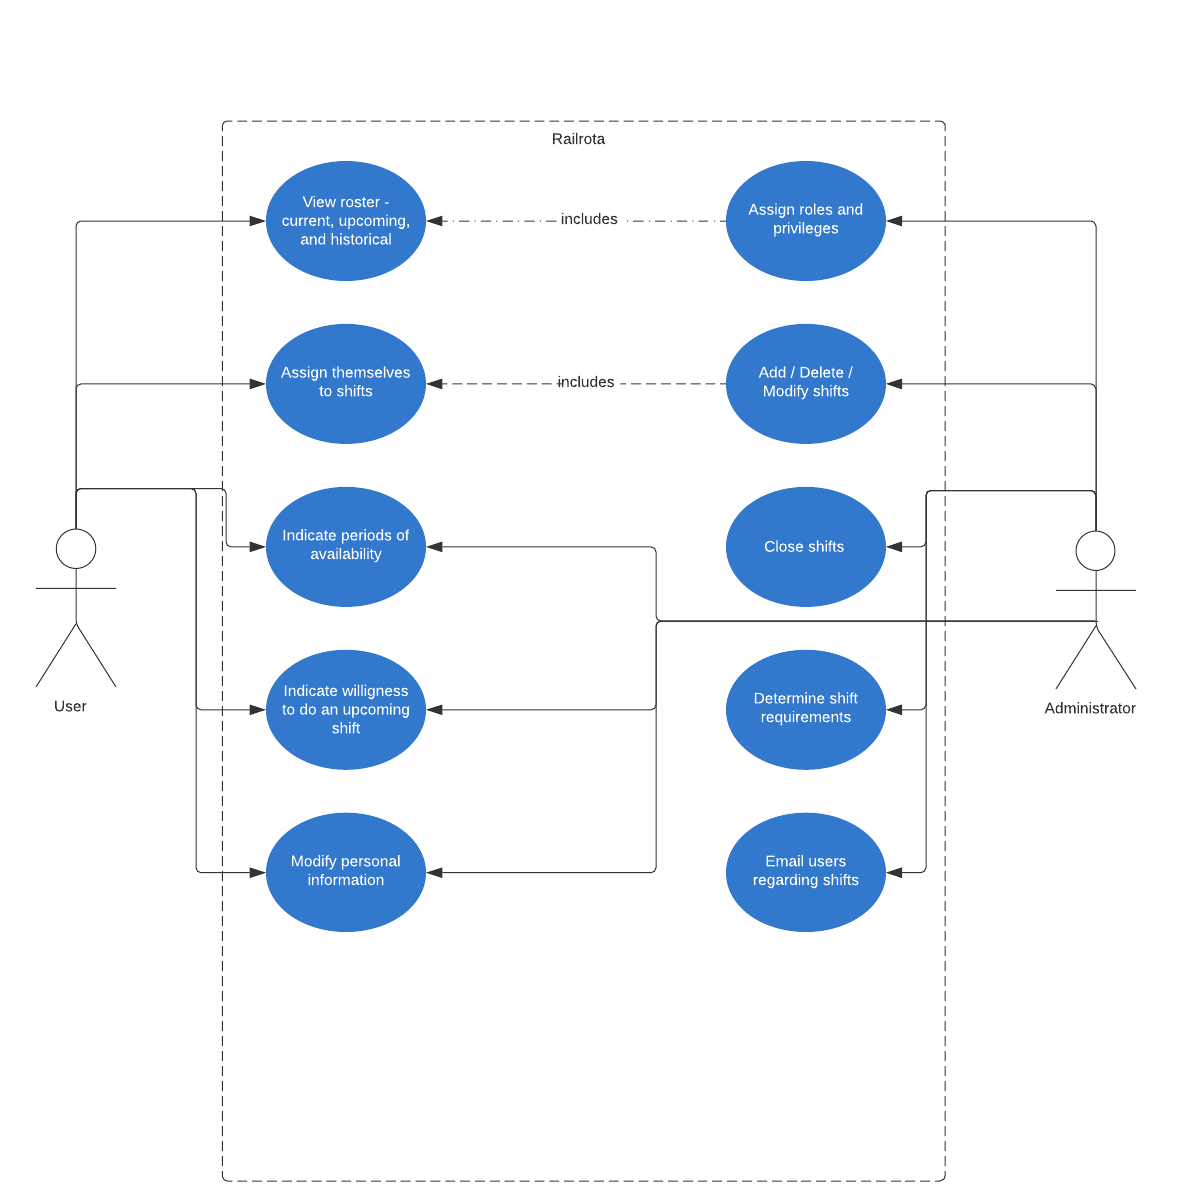
\includegraphics[width=\textwidth]{Figures/usecase}
    \caption{Use Case Diagram.}
    \label{fig:usecase}
\end{figure}

Based on the full requirements list in Chapter 1, there are two primary use cases identified for the application - both for everyday volunteers (users), and administrators. The above diagram shows that the a great deal of functionality is accessible by both user groups, and that administrators have a superset of what could be considered user privileges, such as the ability to add, delete, and modify shifts, in addition to being able to register for a shift. This is because administrators could readily be volunteers themselves and may wish to use the application as such without the need for an additional account.

Users on the other hand, do not have use cases that involve the manipulation of data outside of their own personal information that can and should be updated whenever necessary.

\section{User Interface Design}
The UI design went through two phases - initial sketches done on paper based on initial ideas for how the layout for the application will appear, followed by digital artwork that can be considered the final design before implementation.

In traditional development methodologies, design is something that is done extensively at the start of application development with the final outputs expected to closely resemble the end product. However, agile methodologies, including this Scrum adaptation, recognise that design is a continuous process throughout development, and that the end product may vary vastly from any drawings or early documentation as the result of changing requirements or additional variables such as customer feedback - thus making design a far more cooperative, agile process. \cite{Kiss1}

\subsection{Early Concept Art}
Early concept art can be found in Appendix \ref{Concept Art} due to their large resolutions.

\subsection{Final Iteration}
These rudimentary designs were expanded upon in much more detail that demonstrates a far more mature iteration of the design process.

\subsubsection{Homepage}
\begin{figure}[h]
    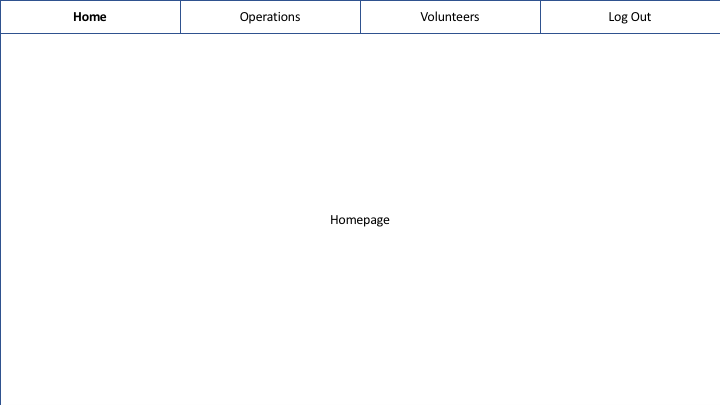
\includegraphics[width=1.0\textwidth]{Figures/design-homepage}
    \caption{Default design of the homepage as viewed on a desktop web browser.}
    \label{fig:homepage}
\end{figure}

The homepage design as visible from desktop viewports provides insight into the UI and how it should appear, most notably showing off the navigation bar.

\subsubsection{Responsive Design}
\begin{figure}[h]
    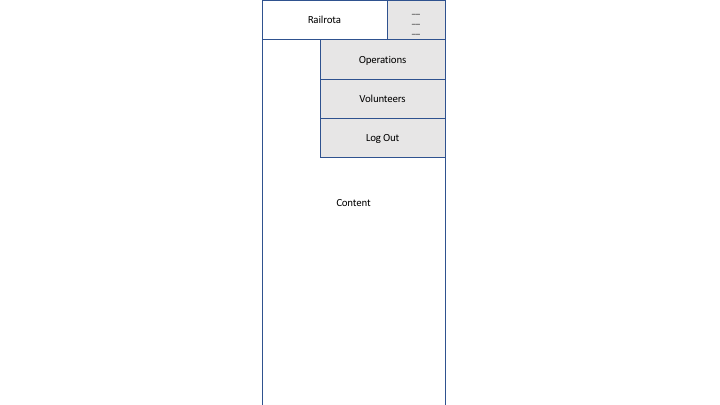
\includegraphics[width=1.0\textwidth]{Figures/design-mobile}
    \caption{Design of how the web application responsively appears in smaller viewports.}
    \label{fig:mobile}
\end{figure}

With the aforementioned emphasis and importance of responsive design and an importance of the design to work and view correctly on mobile devices such as smartphones and tablets, a reduced viewport design was considered important. In particular, this is to demonstrate the use of a collapsable 'hamburger menu', a commonly used dropdown menu optimised for touchscreens, and readily implementable in Bootstrap 4. \cite{Bootstrap4}

\subsubsection{Operations Design}
\begin{figure}[h]
    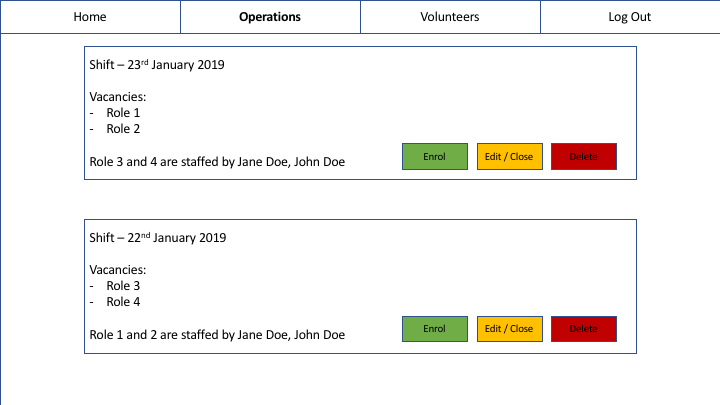
\includegraphics[width=1.0\textwidth]{Figures/design-operations}
    \caption{Design of the operations page that displays operations and shifts.}
    \label{fig:operations}
\end{figure}

This design expands upon the drawing, showing in more detail how each operation might be displayed on the application, with respective information on available shifts, the volunteers either staffing them or whether there are vacancies, and additional buttons for actions on that particular operation.

\subsubsection{Volunteers Design}
\begin{figure}[h]
    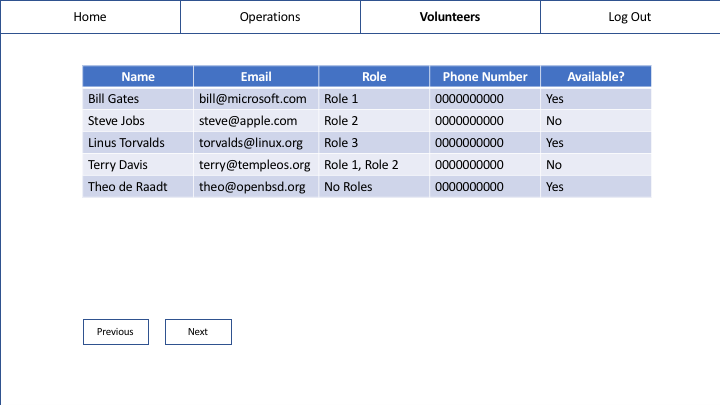
\includegraphics[width=1.0\textwidth]{Figures/design-volunteers}
    \caption{Design of the operations page that displays operations and shifts.}
    \label{fig:volunteers}
\end{figure}

An additional design was drawn up to demonstrate how a tabular view might look, in this instance, displaying a list of volunteers with their personal details, so that a volunteer or an administrator can quickly look up a fellow volunteer and view their public information, such as their availability or contact information.

\subsubsection{Glance / Calendar Design}
\begin{figure}[h]
    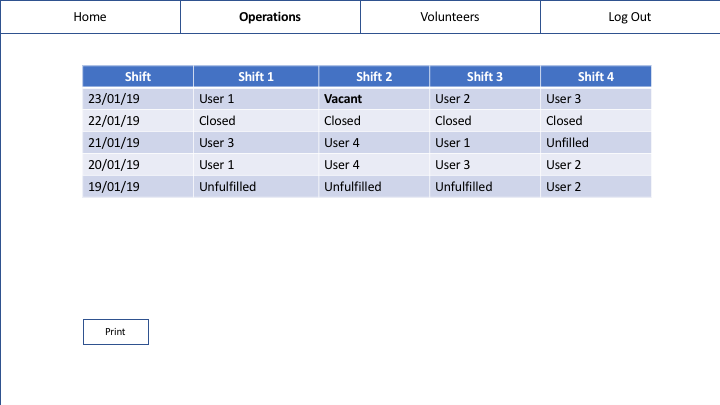
\includegraphics[width=1.0\textwidth]{Figures/design-glance}
    \caption{Design of the more compact operations view, more akin to a calendar.}
    \label{fig:glance}
\end{figure}

Following a conversation with the customer, they expressed a desire to have a view, potentially downloadable and/or printable, that could show 'at a glance' the available shifts and the current staffing at that moment in time. This should somewhat resemble the existing system that is shown in Appendix \ref{Example Timetable}. This is desirable functionality that came into being after development actually began, with the intention in including it into a release of the software, time permitting.
